% ~ 6 pages
\chapter{Theoretical Background}
\label{sec:theory}

\section{The Standard Model}

Dirac equation: describing fermion dynamics\\
Quantum Field Theory: describing particles and their interaction\\
Local gauge principle: determines nature of the interaction\\
Higgs mechanism / electroweak symmetry breaking: generate particle masses\\

Parameters of the Standard Model: 12 fermion masses (Higgs sector), 3 coupling
constants (gauge interactions) $\alpha$, $G_{\text{F}}$, $\alpha_{\text{S}}$,
VEV~$v$ and $m_{\text{H}}$ (Higgs sector), 8 mixing angles of the PMNS and CKM
matrices (flavour sector), CP violating phase of the strong interaction
\cite{thomson}.
Large number of parameters 25 (26 counting the CP violating phase) with 14
related to the Higgs field.

Challenges: Dark matter

Most common high-energy process at the LHC: Production of dijet-events (back to
back in the transverse plane). A lot of QCD diagrams contribute to the dijet
cross-section (qq \textrightarrow qq, qq \textrightarrow gg, gg \textrightarrow
qq, qg \textrightarrow gq, gg \textrightarrow gg, etc.). Dijet cross-section
peaked at low $p_{\text{T}}$.

\section{The Weak \& Strong Interaction}

\section{$\tau$-Leptons}

\todo[inline]{Define 1-prong, 3-prong and multi-prong.}

The tau lepton is the heaviest lepton in the Standard Model and an important
probe of physics at high energy scales, such as Higgs physics and physics beyond
the Standard Model. Hadronic decays make up approximately two-thirds of the
total branching ratio of tau decays and play an important part in the physics
programme of the ATLAS experiment.

\begin{figure}[ht]
  \begin{subfigure}[b]{0.47\textwidth}
    \centering
    \begin{overpic}{./figures/theory/tau_branching_pie_chart.pdf}
      \put (34, 83) {$\pi^- \nu_\tau$}
      \put (-1, 45) {$\pi^- \pi^0 \nu_\tau$}
      \put (19, 8) {$\pi^- 2 \pi^0 \nu_\tau$}
      \put (44.5, 2) {$2 \pi^- \pi^+ \nu_\tau$}
      \put (69, 6) {$2 \pi^- \pi^+ \pi^0 \nu_\tau$}
      \put (80, 15) {other}
    \end{overpic}
    \caption{Tau branching ratios \cite{pdg}. Adapted from
      Ref.~\cite{ikai_trigger}.}
    \todo[inline]{Fix wonky percentages for hadronic modes}
    \label{fig:tau_branching_ratios}
  \end{subfigure}\hfill
  \begin{subfigure}[b]{0.47\textwidth}
    \centering
    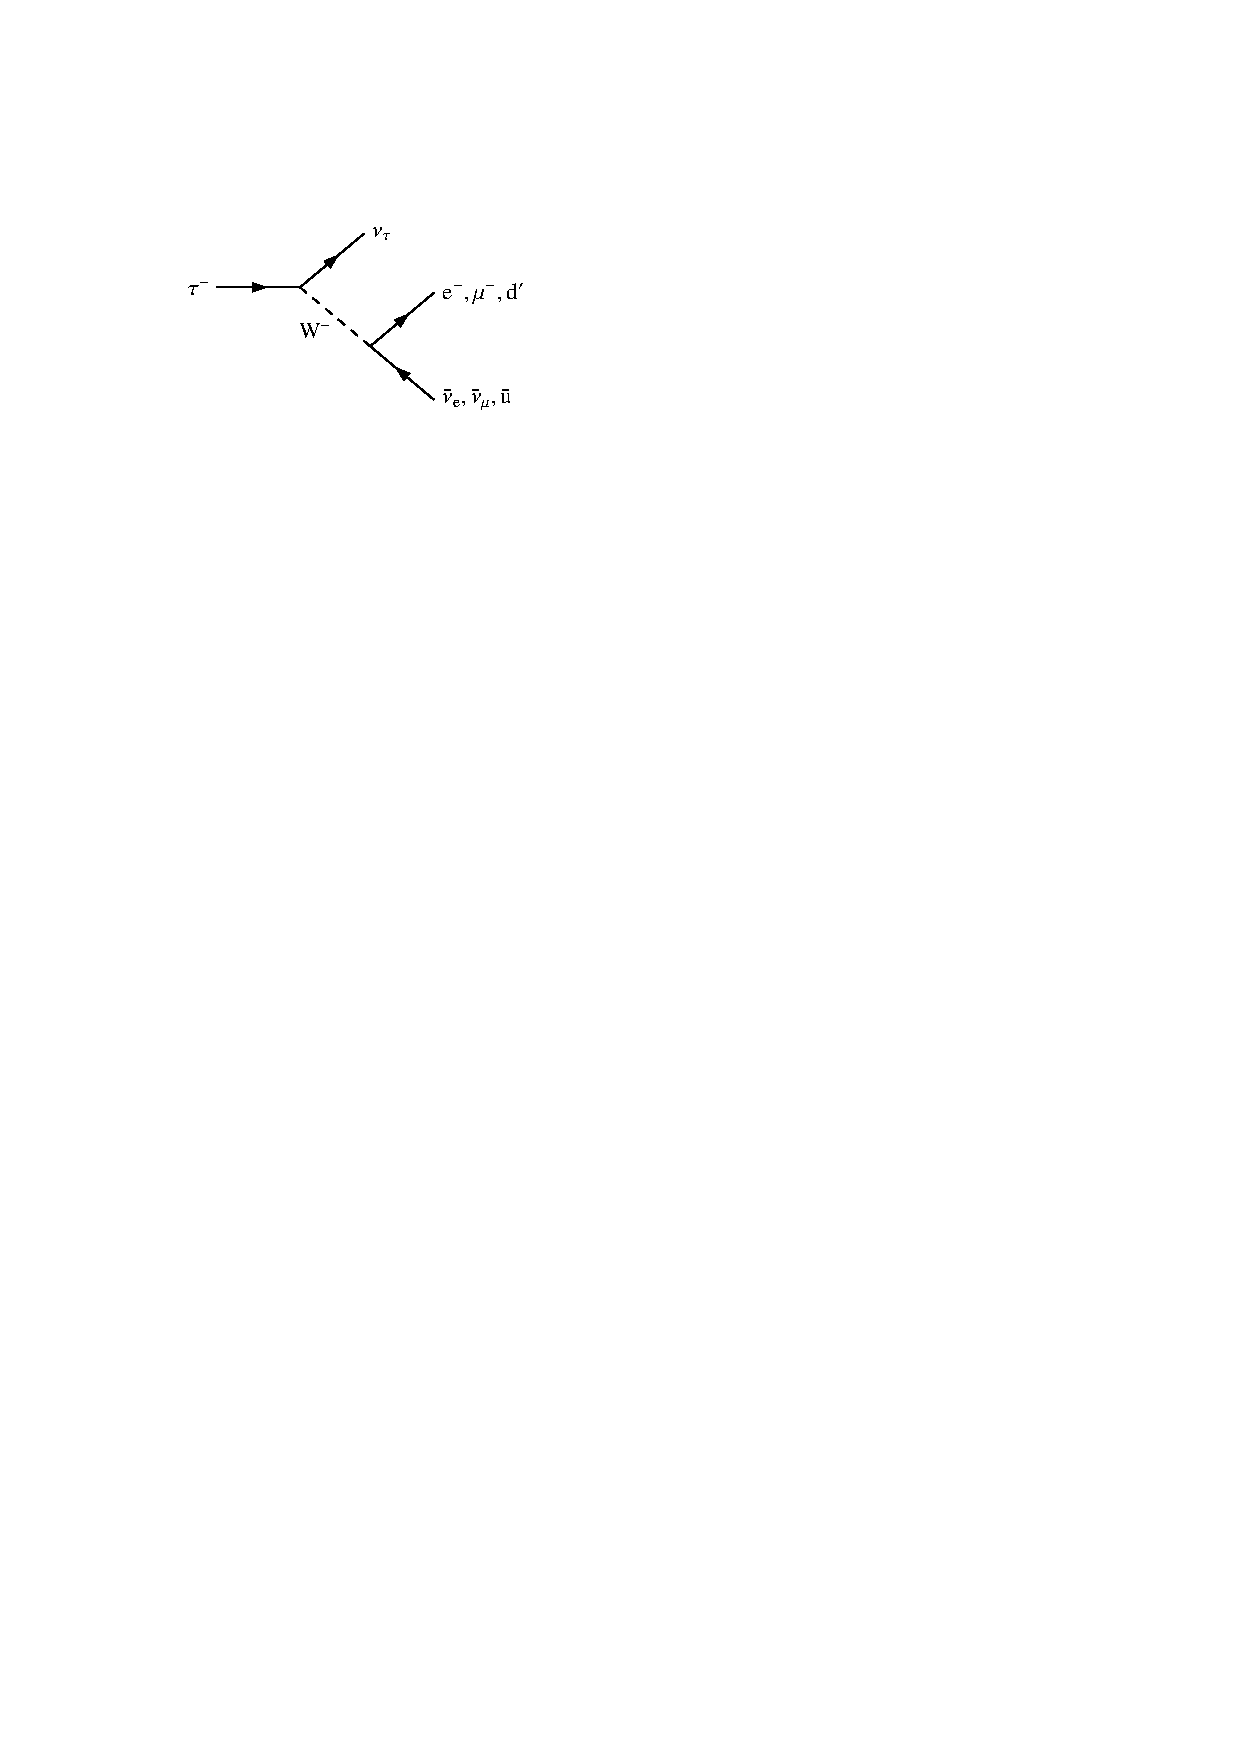
\includegraphics{./figures/theory/tau_decay_feynman.pdf}
    \caption{Feynman Diagram. Strangeness production is Cabibbo suppressed by a
      factor of $\sin^2\theta_\mathrm{c} / \cos^2\theta_\mathrm{c} \approx
      \frac{1}{20}$. Ignoring phase space considerations the tau decays to
      $\frac{1}{5}$ into electron or muon and corresponding antineutrino or into
      a down anti-up quark pair (3 colours).}
  \end{subfigure}
  \caption{Weak decay of the tau-lepton}
\end{figure}

\begin{itemize}
\item Discovery at SPEAR in 1975 [Check Citation]\cite{perl}
\item $m_\tau = \SI{1776.86 +- 0.12}{\mega\electronvolt}$ \cite{pdg}
\item Tau more than twelve times heavier than pions \textrightarrow can decay
  into quark-antiquark pairs (strangeness production cabbibo suppressed)
\item 5 possible weak decay modes: electron (20\%), muon (20\%), ud (3 times
  20\% due to 3 color charges) -- ignoring phase space
\item unit charge \textrightarrow decays into odd number of charged particles
  (prong definition)
\item Two or three pion modes mainly through intermediate $\rho$ or $a_1$
  resonances
\item Charged pion 'stable' and showers in the HCAL
\item Neutral pion decays immediately into two photons which shower in the ECAL.
  Created photons often convert into an electron positron pair in the presence
  of material
\end{itemize}

\todo[inline]{Introduce \tauhad and \tauhadvis notation}

\section{Features of Hadronically Decaying Tau Leptons}
\label{sec:features_tau_decay}

\todo[inline]{Signature of the decay modes}

\todo[inline]{Leptonic decays of the tau are identified using the electron/muon
  identification.}

Features of hadronically decaying $\tau$-leptons vs. Quark/Gluon initiated jets:
\begin{itemize}
\item Low multiplicity (QCD jets usually have a lot of tracks)
\item Isolated tracks and narrow showers
\item Measurable decay length with proper lifetime of
  $\tau = \SI{290.3 +- 0.5}{\femto\second}$ \cite{pdg} and following from that
  $c \tau = \SI{87.0 +- 0.2}{\micro\metre}$ with $\beta \gamma = 10$ which
  corresponds to a roughly \SI{18}{\giga\electronvolt} tau the mean decay length
  is of the order of a millimetre and allows secondary vertex reconstruction or
  employing the impact parameter for 1-prong taus (sub-millimetre resolution).
\item Invariant mass bounds for decay products
\item $\pi^0$ content???
\end{itemize}

% ----------------------- FIRST DRAFT ---------------------- %
\begin{itemize}

\item The Standard Model
  \begin{itemize}
  \item Features \& Successes

  \item Challenges (neutrino masses, dark matter, matter-antimatter asymmetry,
    gravitation, number of parameters, hierarchy problem, \ldots)

  \item Beyond the Standard Model (SUSY -- preferred coupling to down-type
    fermions for large $\tan\beta$ \textrightarrow $\tau$-leptons)
  \end{itemize}

\item Weak Interaction
\begin{itemize}
\item Can be kept very short. Only whats necessary to understand Tau-ID
\end{itemize}

\item Strong Interaction
\begin{itemize}
\item Can be kept very short. Only whats necessary to understand Tau-ID
\item Confinement \& Hadronization
\item Quark \& Gluon initiated jets
\end{itemize}

\item $\tau$-Leptons
\begin{itemize}
\item Discovery

\item Properties (mass \textrightarrow lep \& had, mean life time
  \textrightarrow no direct detection)

\item Hadronically Decaying $\tau$-Leptons
  \begin{itemize}
  \item Feynman Diagram, Decay Modes (interm. resonances) \& Branching Ratios
    (pie chart like in: \url{https://www.lhc-ilc.physik.uni-bonn.de/ergebnisse/dateien/t00000078.pdf?c=t&id=78}
    on p.\ 25)
  \item Detector signature ($\pi^0$ ($\gamma \gamma$ / $\mathrm{e}^+
    \mathrm{e}^- \gamma$), $\pi^\pm$ ($\mathrm{K}^\pm$), $\nu_\tau$,
    conversions)
  \item Jets faking taus
  \end{itemize}

\item $\tau$ Physics
  \begin{itemize}
  \item $\mathrm{Z} \rightarrow \tau \tau$ (background for H$\tau \tau$ and
    useful for performance measurements using tag-and-probe -- semileptonic
    decays)

  \item $\mathrm{H} \rightarrow \tau \tau$ (one of two channels to measure
    the fermionic coupling -- $b \bar{b}$ plagued by multijet background,
    Higgs CP)

  \item MSSM Higgs (potentially high branching fraction to $\tau$-leptons)

  \item $\mathrm{Z}^\prime$ could preferentially decay into third-generation
    fermions (lepton universality not required).

  \item $\mathrm{W}^\prime$ models with preferential coupling to third-gen.

  \item SUSY with $\tau$ \textrightarrow long decay chains
  \end{itemize}
\end{itemize}
\end{itemize}

% -----------------------------???-------------------------- %

\begin{itemize}
\item Tau lepton

\item Weak \& strong interaction (?)
  \begin{itemize}
  \item Cross section plot multijet (large cross section) vs.
    electroweak interaction (small)
  \item \url{http://www.hep.ph.ic.ac.uk/~wstirlin/plots/plots.html}
  \item Quark vs Gluon jets: \url{http://jets.physics.harvard.edu/qvg/}
    Because of different colour interaction and hadronization, gluon jets are
    wider, with higher multiplicity and have a more uniform energy
    fragmentation, while quark jets are more likely to produce narrow jets with
    hard constituents that carry a significant fraction of the energy.
  \end{itemize}

\item Tau decay modes \& branching fractions
  \begin{itemize}
  \item Hadronic decays not containing pions but kaons etc.
  \end{itemize}

\item Intermediate resonances $a$, $\rho$

\item Jets (anti-$k_\mathrm{T}$)

\end{itemize}

%%% Local Variables:
%%% mode: latex
%%% TeX-master: "mythesis"
%%% End:
